SAT solver is described by the following pipeline. \vspace{3.5pt}
\begin{center}
    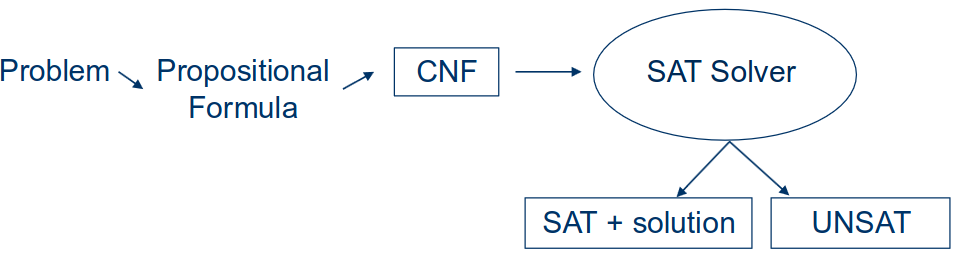
\includegraphics[width = 0.7 \textwidth]{img/img28.png}
\end{center} \vspace{3.5pt}
Before moving on, let's take a look at the image above:
\begin{enumerate}
    \item Problem $\rightarrow$ Propositional formula: translation of the original problem to a boolean formula.
    \item Propositional formula $\rightarrow$ CNF: conversion of the boolean formula to an intermediate form, called Conjuctive Normal Form (\textit{CNF}), conjuction of disjuctions.
    \item CNF $\rightarrow$ SAT solver: CNF boolean formula given to the SAT solver.
    \item SAT solver $\rightarrow$ SAT + Solution $\vee$ UNSAT: SAT solver gives us the final solution of the original problem.
\end{enumerate}
The first step (\textit{Problem $\rightarrow$ Propositional formula}) of the SAT solver pipeline is called the \textbf{encoding} phase, while the second part 
from \textit{Propositional $\rightarrow$ CNF} to \textit{SAT solver} $\rightarrow$ \textit{Final answer} is the \textbf{solving} phase.